Im Folgenden wird  anhand eines Beispiels gezeigt, wie  der Arbeitsprozess mit
unserer  Software funktioniert. Dabei  werden wir  sowohl einen  PI-Regler als
auch einen PID-Regler durchrechnen und den Prozess grafisch illustrieren.

Als  Ausgangspunkt  des  Prozesses   dient  die  Schrittantwort  der  Strecke,
aus  welcher  die  Verts\"arkung  $K_s$ der  Strecke,  die  Verz\"ogerungszeit
$T_u$  und die  Anstiegszeit $T_g$  abgelesen werden. Diese  Werte dienen  als
Eingabeparameter unseres Tools.

Wir werden in diesem Bericht folgende Strecke als Beispiel nehmen:
\begin{figure}[h! width=\pagewidth]
    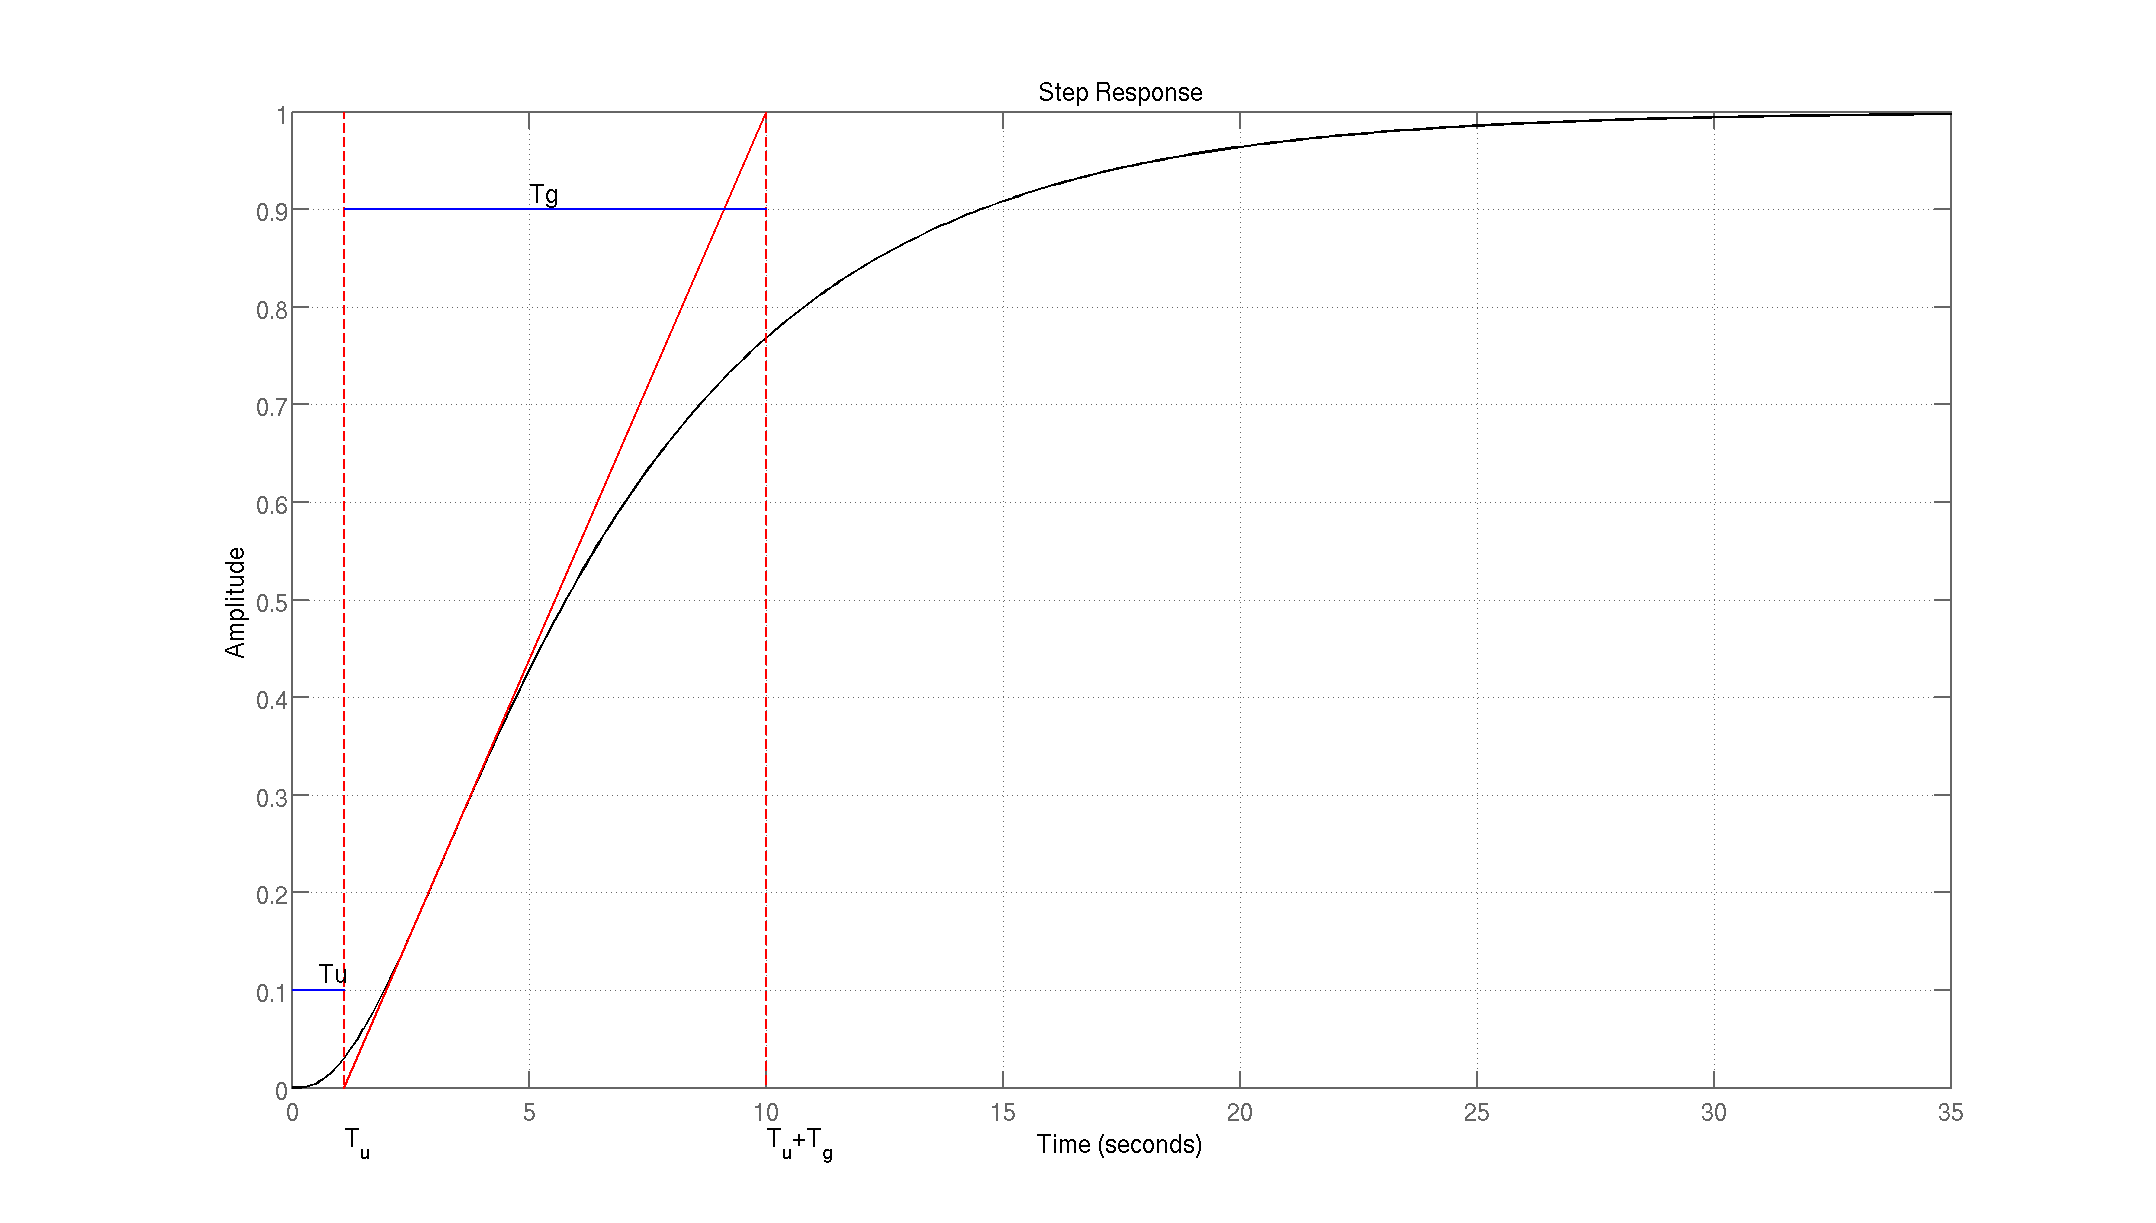
\includegraphics[width=\textwidth]{images/streckeSchrittantwort.png}
    \caption{%
    Schrittantwort der  Beispielstrecke (schwarz), Wendetangende  (rot), $T_u$
    und $T_g$ (blau)%
    }
    \label{fig:plant_step}
\end{figure}

Der  geschlossene   Regelkreis  soll  schlussendlich  maximal   etwa  $16.3\%$
\"uberschwingen.

Wir erhalten:
\begin{itemize}
    \item
        $K_s = \SI{2}{\second}$
    \item
        $T_u = \SI{1.1}{\second}$
    \item
        $T_g = \SI{8.9}{\second}$
\end{itemize}

Da  die Phasengangmethode  vom {\em{Frequenzgang}}  einer Strecke  ausgeht und
nicht von der Schrittantwort, besteht der n\"achste Schritt nun darin, aus den
obigen Werten  den Frequenzgang  der Strecke  zu bestimmen. Dies  erledigt die
Methode \code{p\_sani}, welche uns  die Werte f\"ur die \"Ubertragungsfunktion
der  Strecke   liefert.  \todo{Allenfalls   Verweis  auf   Softwareteil  f\"ur
Erkl\"arungen  zu  sani-Methode.}   In  unserem  Fall  ergibt  dies  folgendes
Polynom:

\begin{gather} \label{eq:transfer:plant}
    \begin{split}
        H_s (s) & = K_s
                  \cdot \frac{1}{1 + s \cdot T_1}
                  \cdot \frac{1}{1 + s \cdot T_2}
                  \cdot \frac{1}{1 + s \cdot T_2}                     \\
                & = 2
                  \cdot \frac{1}{1 + s \cdot \SI{0.4134}{\second}}
                  \cdot \frac{1}{1 + s \cdot \SI{1.4894}{\second}}
                  \cdot \frac{1}{1 + s \cdot \SI{5.3655}{\second}}
    \end{split}
\end{gather}

Mit einem  geeigneten Tool  kann man sich  den dazugeh\"origen  Plot erstellen
lassen.

\begin{figure}[h! width=\pagewidth]
    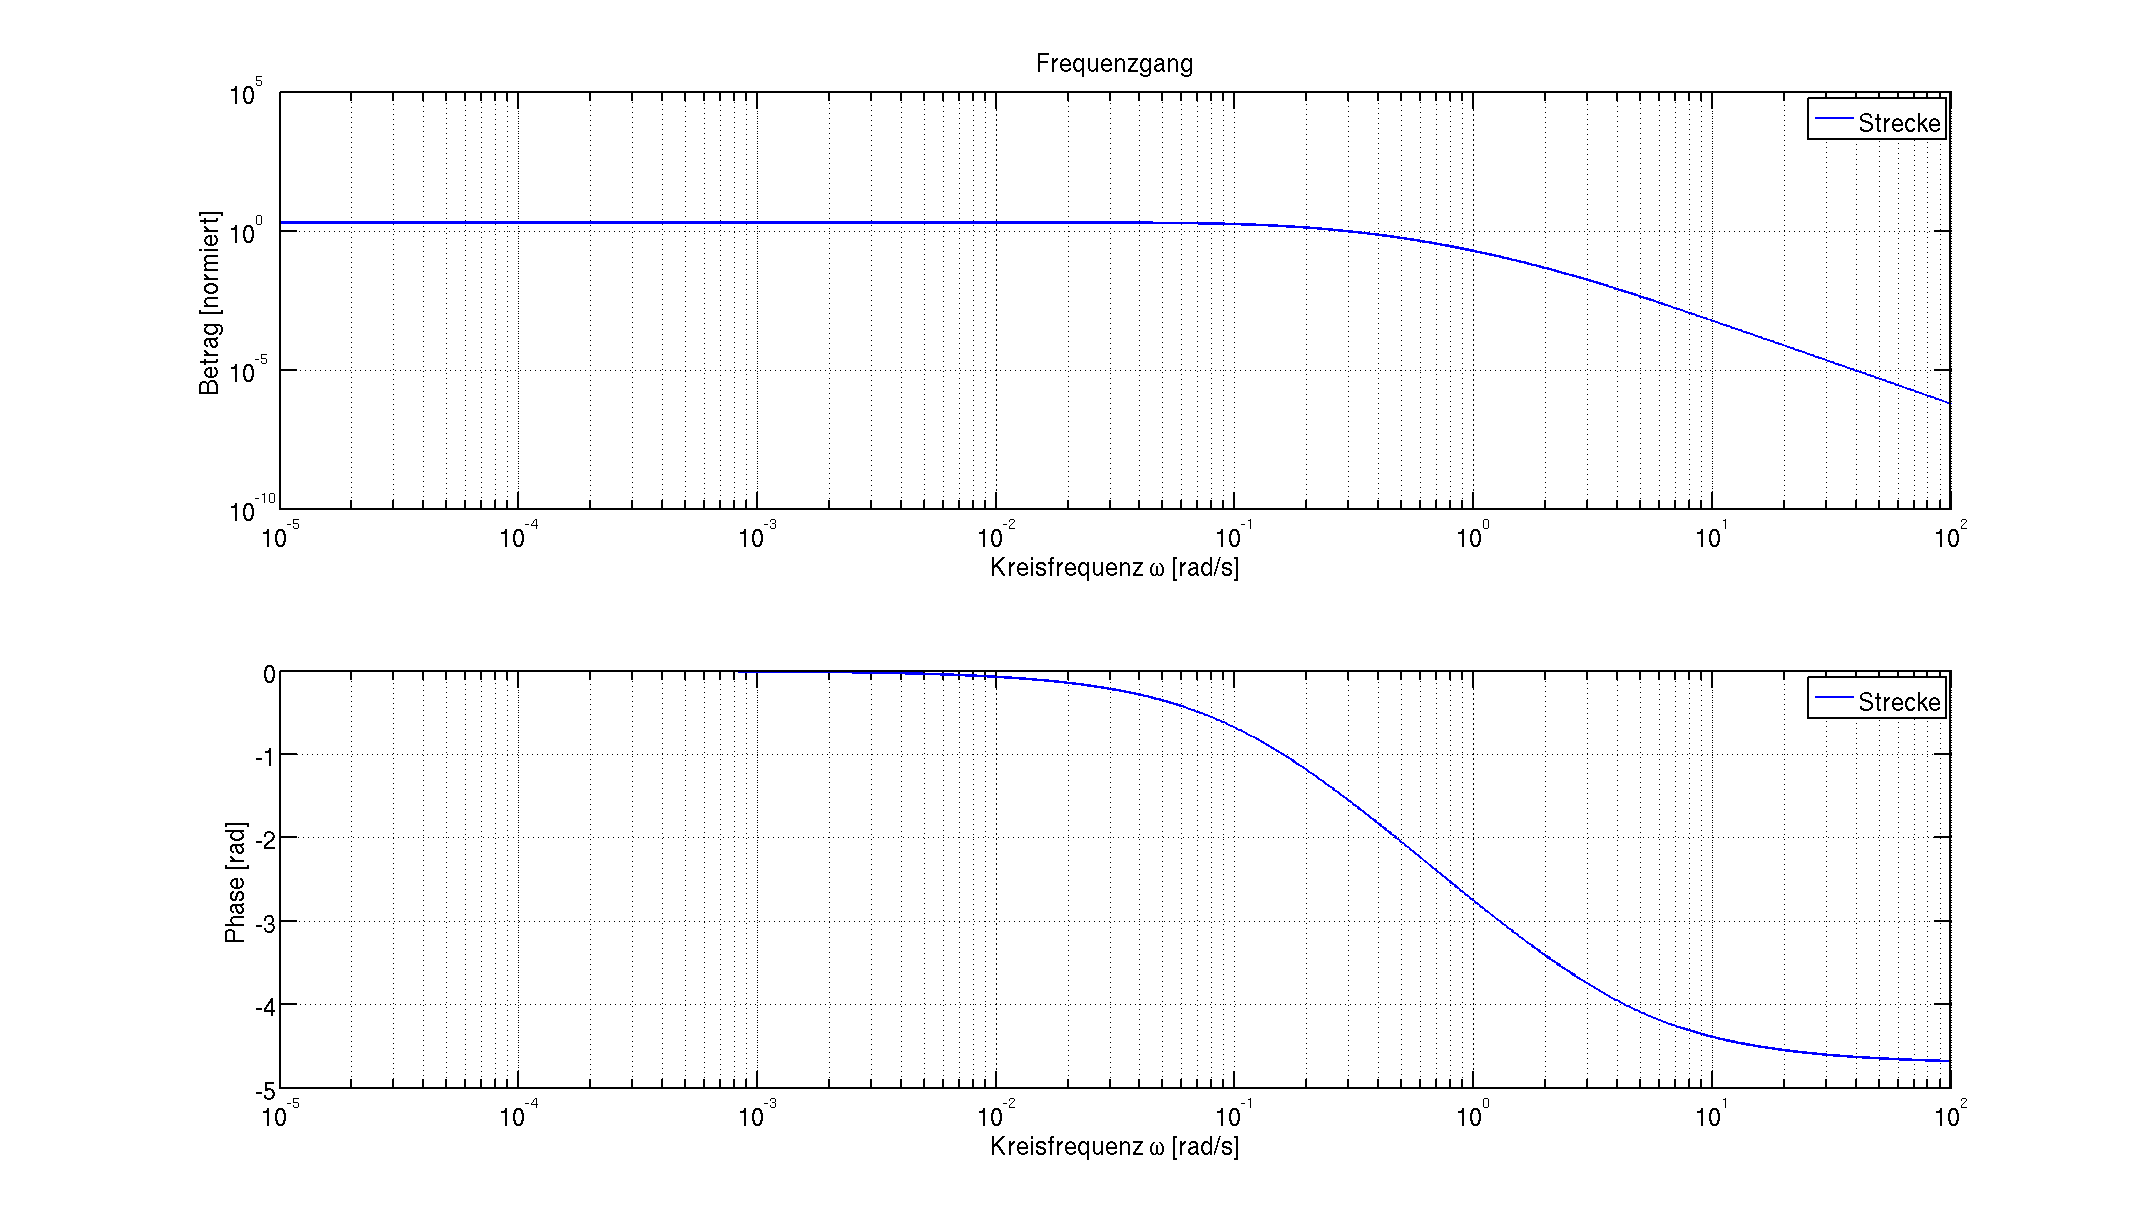
\includegraphics[width=\textwidth]{images/streckeFrequenzgang.png}
    \caption{%
        Frequenzgang der Strecke%
    }
    \label{fig:plant_freq}
\end{figure}

An diesem Punkt divergieren die Verfahren f\"ur den PI- und den PID-Regler. Es
soll zuerst der PI-Regler dimensioniert werden.

\subsubsection*{PI-Regler}

Das  Ziel ist  die  Bestimmung  der Parameter  $K_{rk}$  und  $T_{nk}$ in  der
Gleichung:

\begin{equation} \label{eq:pi:target}
    H_{rpi} = K_{rk} \cdot \biggl[ 1 + \frac{1}{s \cdot T_{nk}} \biggr]
\end{equation}

Zuerst wird im Phasengang der Strecke die Frequenz $\omega_{pi}$ bestimmt, f\"ur
welche die Phase der Strecke $-90\degree$ betr\"agt.

\begin{equation} \label{eq:pi:phi_s}
    \varphi_s(\omega_{pi}) = -90 \degree
\end{equation}

\begin{figure}[h! width=\pagewidth]
    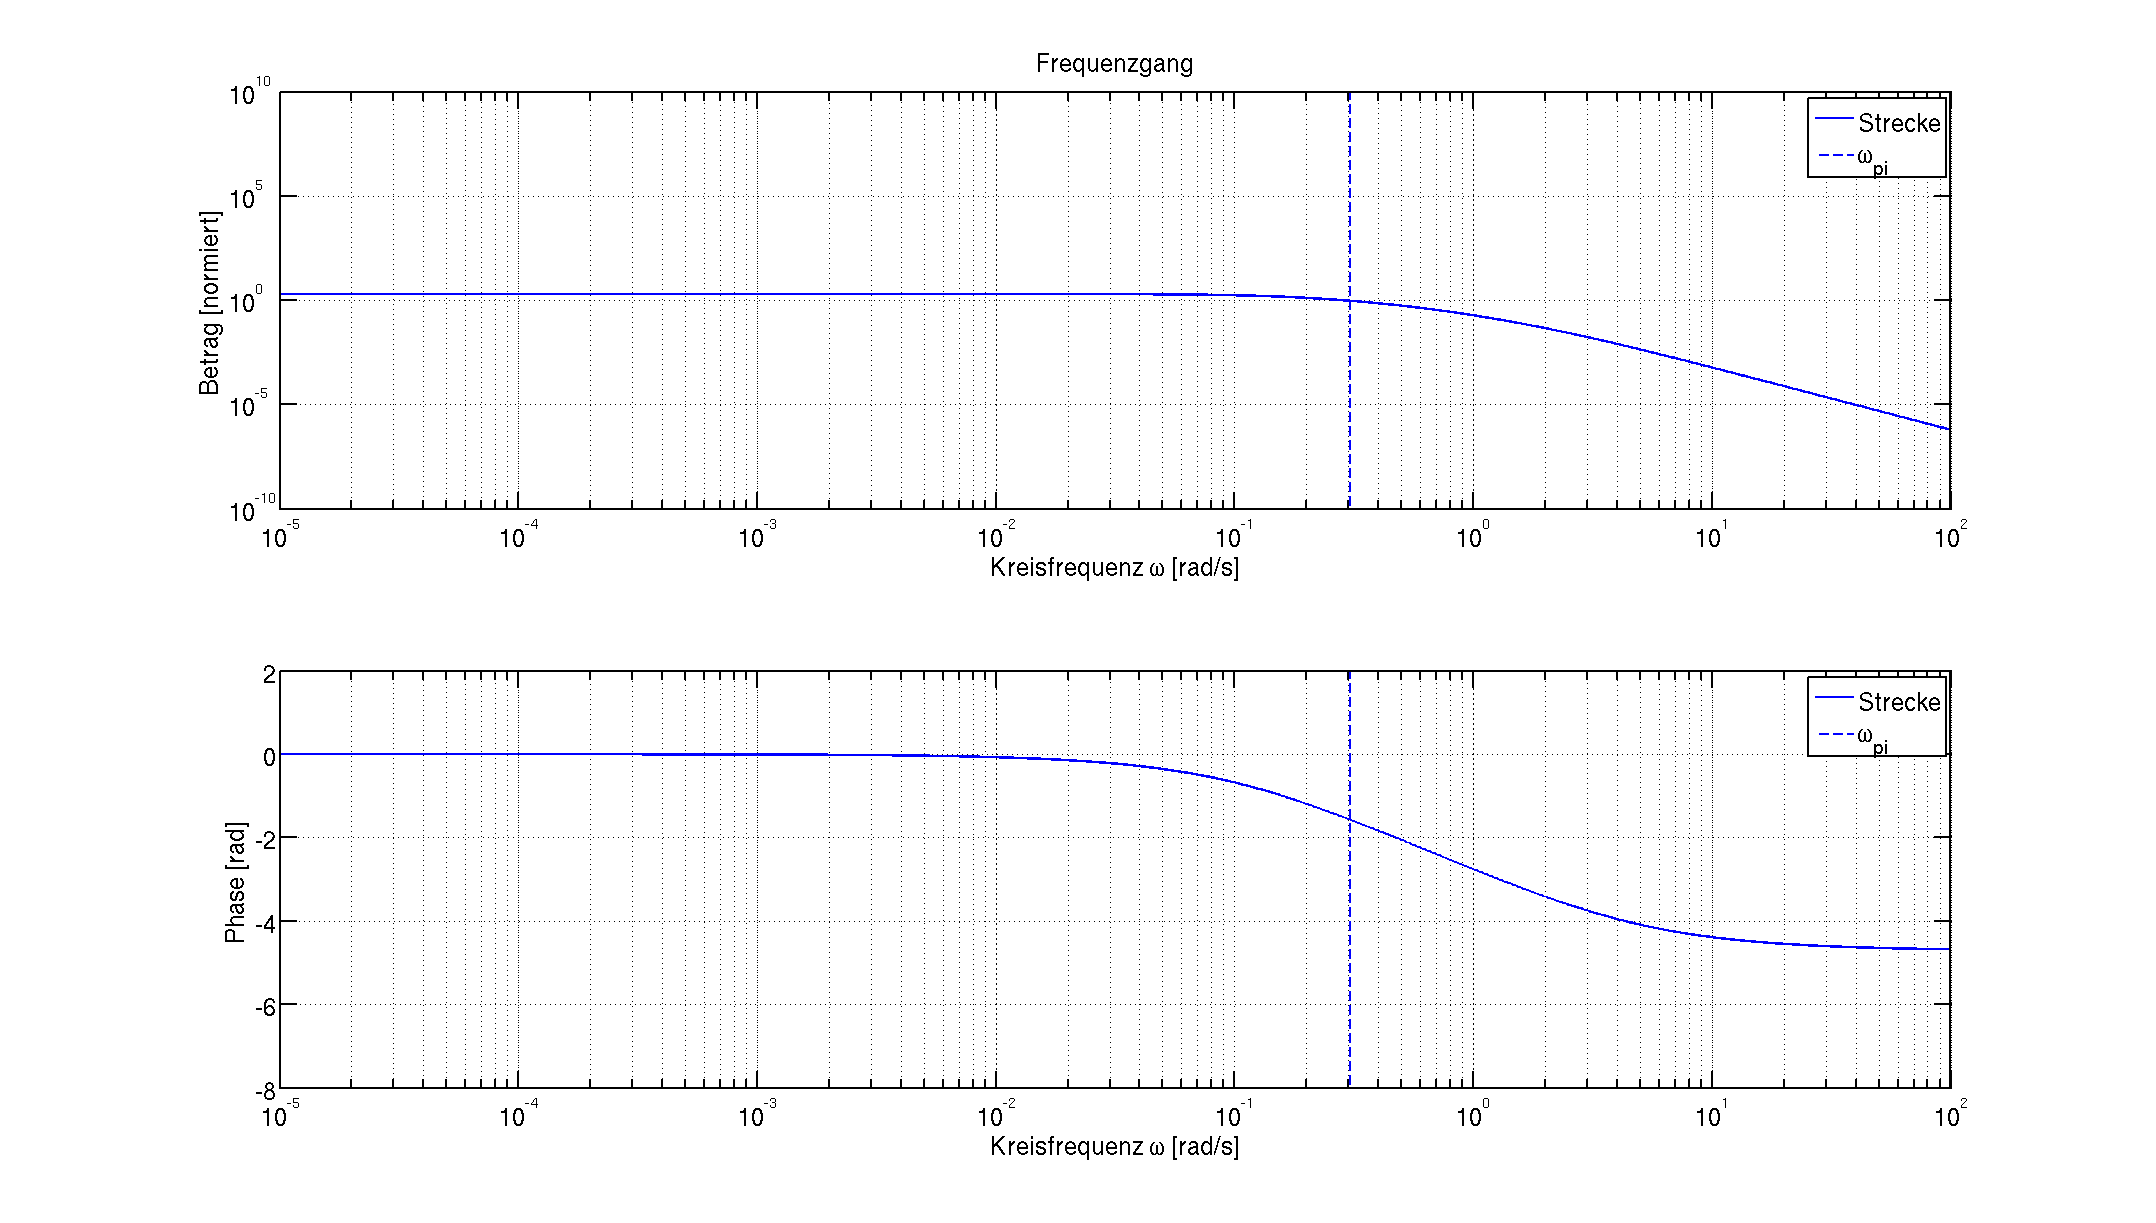
\includegraphics[width=\textwidth]{images/piStreckeOmegaPI.png}
    \caption{%
        $\omega_{pi}$ eingetragen (vertikale gestrichelte Linie).
    }
    \label{fig:pi:omega_pi}
\end{figure}

Wie man aus Abbildung \ref{fig:pi:phi_s} ablesen kann, liegt dieser Wert f\"ur
$\omega_{pi}$ in unserem  Beispiel bei ungef\"ahr $\SI{0.3}{\per\second}$. Die
Kontrollrechnung mittels Matlab ergibt:

\begin{equation} \label{eq:pi:omega_pi}
    \omega_{pi} = \SI{0.3039}{\per\second}
\end{equation}

Damit kann nun $T_{nk}$ direkt bestimmt werden\footnotemark[1]:

\begin{equation} \label{eq:pi:omega_pi}
    T_{nk} = \frac{1}{\omega_{pi}} = \frac{1}{\SI{0.3039}{\per\second}} = \SI{3.2902}{\second}
\end{equation}

\footnotetext[1]{
    Um die  Akkumulation von Ungenauigkeiten  zu minimieren werden  bei diesen
    Berechnungen  die  genauen  Werte  aus  Matlab  verwendet  und  nicht  die
    gerundeten  Zwischenresultate,  was  zu   Abweichungen  zu  den  von  Hand
    berechneten Ergebnissen f\"uhren kann.
}
\todo{Fragen ob dies OK ist.}

Als N\"achstes  soll die Durchtrittsfrequenz $\omega_d$  bestimmt werden. Dazu
wird  der  f\"ur  $T_{nk}$  erhaltene  Wert  in  Gleichung  \ref{eq:pi:target}
eingesetzt. Da $K_{rk}$ noch unbekannt ist, wird vorerst $K_{rk} = 1$ gesetzt.

\begin{gather} \label{eq:pi:target}
    \begin{split}
        H_{rpi} & = K_{rk} \cdot \biggl[ 1 + \frac{1}{s \cdot T_{nk}} \biggr] \\
                & = 1      \cdot \biggl[ 1 + \frac{1}{s \cdot \SI{3.2902}{\second}} \biggr]
    \end{split}
\end{gather}

Daraus   kann   nun   der   Frequenzgang   des   {\em{offenen   Regelkreises}}
(\"Ubertragungsfunktion $H_o$,  Amplitudengang $A_o$,  Phasengang $\varphi_o$)
bestimmt werden.

\begin{gather} \label{eq:pi:h_open}
    \begin{split}
        H_o (s) & = H_{rpi} (s) \cdot H_s (s) \\
            & = \Biggl(
                    K_{rk} \cdot \biggl[ 1 + \frac{1}{s \cdot T_{nk}} \biggr]
                \Biggr)
                \cdot
                K_s
                \cdot
                \Biggl(
                        \frac{1}{1 + s \cdot T_1}
                  \cdot \frac{1}{1 + s \cdot T_2}
                  \cdot \frac{1}{1 + s \cdot T_2}
                \Biggr) \\
            & = \Biggl(
                    1 \cdot \biggl[ 1 + \frac{1}{s \cdot \SI{3.2902}{\second}} \biggr]
                \Biggr)
                \cdot
                2
                \cdot
                \Biggl(
                          \frac{1}{1 + s \cdot \SI{0.4134}{\second}}
                    \cdot \frac{1}{1 + s \cdot \SI{1.4894}{\second}}
                    \cdot \frac{1}{1 + s \cdot \SI{5.3655}{\second}}
                \Biggr)
    \end{split}
\end{gather}


Wobei der Amplitudengang den Betragsverlauf und der Phasengang den Verlauf des
Arguments dieser \"Ubertragungsfunktion repr\"asentieren:
\todo{Allenfalls auch wirklich ausrechnen... w\"urde aber ziemlich langwierig.}

\begin{equation}
    \begin{split} \label{eq:pi:a_o_phi_o}
        A_o(j\omega)       & = |H_o(j\omega)| \\
        \varphi_o(j\omega) & = arg(H_o(j\omega))
    \end{split}
\end{equation}

Von besonderem  Interesse ist  hier der Phasengang. Wie  Anfangs spezifiziert,
soll  ein maximals  \"Uberschwingen von  ca. $16.3\%$ angestrebt  werden. Dazu
muss die Durchtrittsfrequenz $\omega_d$ gefunden werden, an welcher der offene
Regelkreis eine Phase von $-128.5\degree$ aufweist. \footnotemark[2]

\footnotetext[2]{%
    Wird ein anderes \"Uberschwingverhalten gew\"unscht, muss hier ein anderer
    Wert f\"ur die Durchtrittsfrequenz  $\omega_d$ bestimmt werden, siehe dazu
    Tabelle \ref{tab:phi_s}.
}

\begin{figure}[h! width=\pagewidth]
    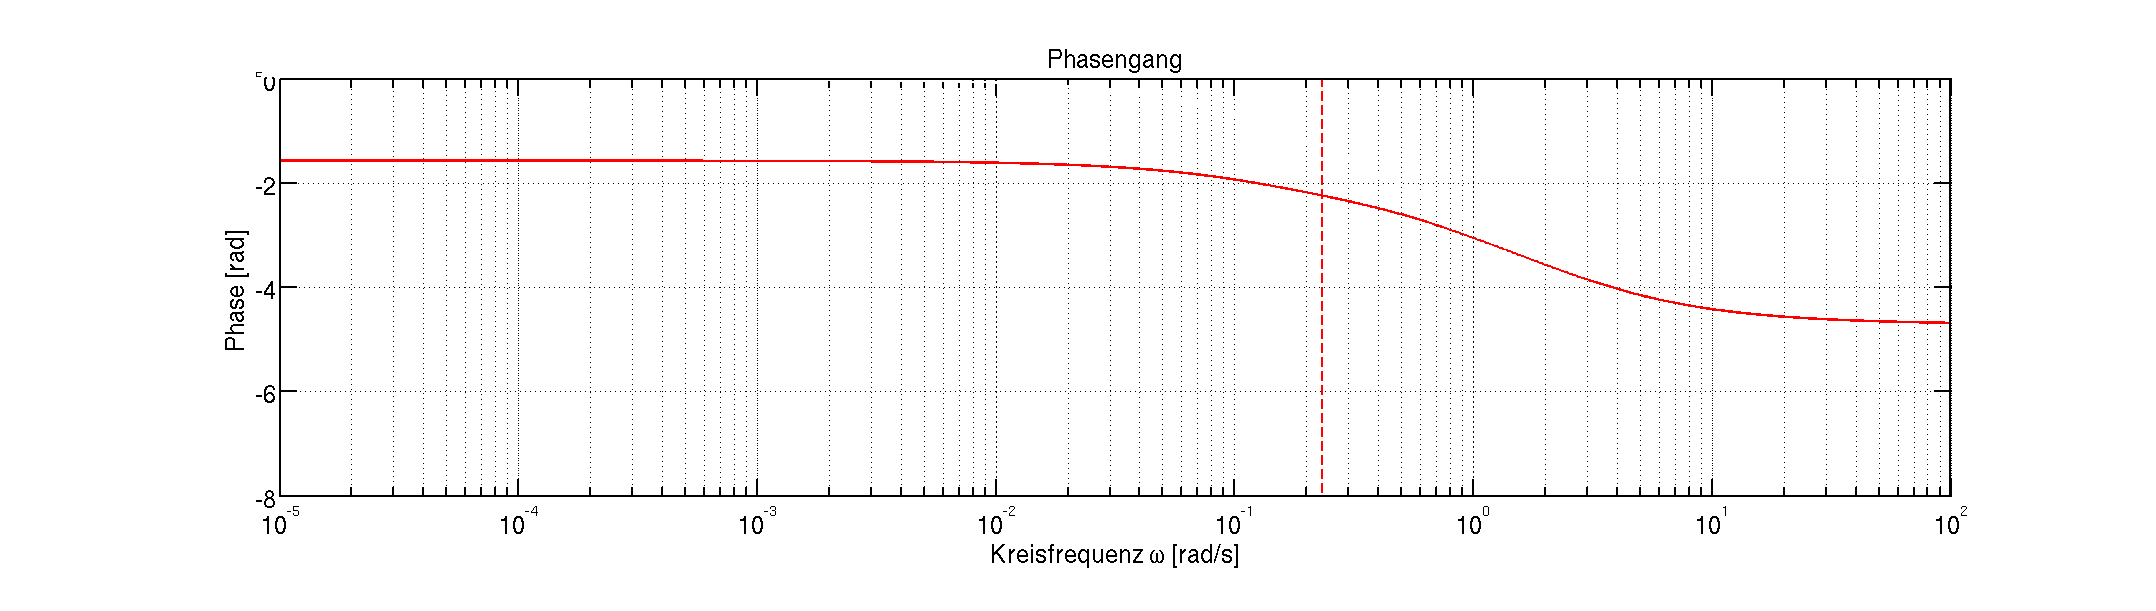
\includegraphics[width=\textwidth]{images/piOffenerRegelkreisPhasengang.png}
    \caption{%
        Phasengang   $\varphi_o(j\omega)$   des   offenen   Regelkreises   mit
        eingetragener Durchtrittsfrequenz $\omega_{d}$ (vertikale gestrichelte
        Linie). Wie man verifizieren kann, weist der offene Regelkreis unseres
        Beispiels bei dieser Kreisfrequenz  eine Phase von $-128.5\degree$ auf
        (etwa $\SI{-2.24}{\radian}$).
    }
    \label{fig:pi:omega_d}
\end{figure}

Dies ergibt:
\begin{equation} \label{eq:pi:omega_d}
    \omega_d = \SI{0.2329}{\per\second}
\end{equation}

In  einem  letzten  Schritt  wird  nun  die  Durchtrittsfrequenz  benutzt,  um
die  ben\"otigte Verst\"arkung  $K_{rk}$ des  Reglers zu  bestimmen. Dazu wird
$\omega_d$ in  Gleichung \ref{eq:pi:h_open}  eingesetzt, $|H_o(j\omega)|  = 1$
gesetzt    (Durchtrittsfrequenz: Frequenz,     bei    der     die    Amplitude
$\SI{0}{\decibel} = 1$ ist).

\begin{gather} \label{eq:pi:A_o_set_to_one}
    \begin{split}
        A_o & = | H_o (j\omega_d) | \\
            & = \abs*{
                    \bigg(
                        K_{rk} \cdot \biggl[ 1 + \frac{1}{j \cdot \omega_d \cdot T_{nk}} \biggr]
                    \bigg)
                    \cdot
                    K_s
                    \cdot
                    \bigg(
                            \frac{1}{1 + j \cdot \omega_d \cdot T_1}
                      \cdot \frac{1}{1 + j \cdot \omega_d \cdot T_2}
                      \cdot \frac{1}{1 + j \cdot \omega_d \cdot T_2}
                      \bigg)} \\
              & = 1
    \end{split}
\end{gather}

Mit den Werten
\begin{equation} \label{eq:pi:values}
    \begin{split}
        K_s      & = 2                    \\
        T_{nk}   & = \SI{3.2902}{\second} \\
        T_1      & = \SI{0.4134}{\second} \\
        T_2      & = \SI{1.4894}{\second} \\
        T_3      & = \SI{5.3655}{\second} \\
        \omega_d & = \SI{0.2329}{\radian\per\second}
    \end{split}
\end{equation}

l\"ost  man Gleichung  \ref{eq:pi:A_o_set_to_one}  nun nach  $K_{rk}$ auf  und
erh\"alt:

\begin{equation} \label{eq:pi:k_rk_result}
    K_{rk} = 0.517577
\end{equation}

Somit ist der PI-Regler vollst\"andig bestimmt und hat folgende Form:

\begin{equation} \label{eq:pi:result}
    H_{rpi} = 0.518 \cdot \biggl[ 1 + \frac{1}{s \cdot \SI{3.29}{\second}} \biggr]
\end{equation}

Zum Vergleich das Bode-Diagramm mit allen relevanten Kurven und Werten:
\begin{figure}[h! width=\pagewidth]
    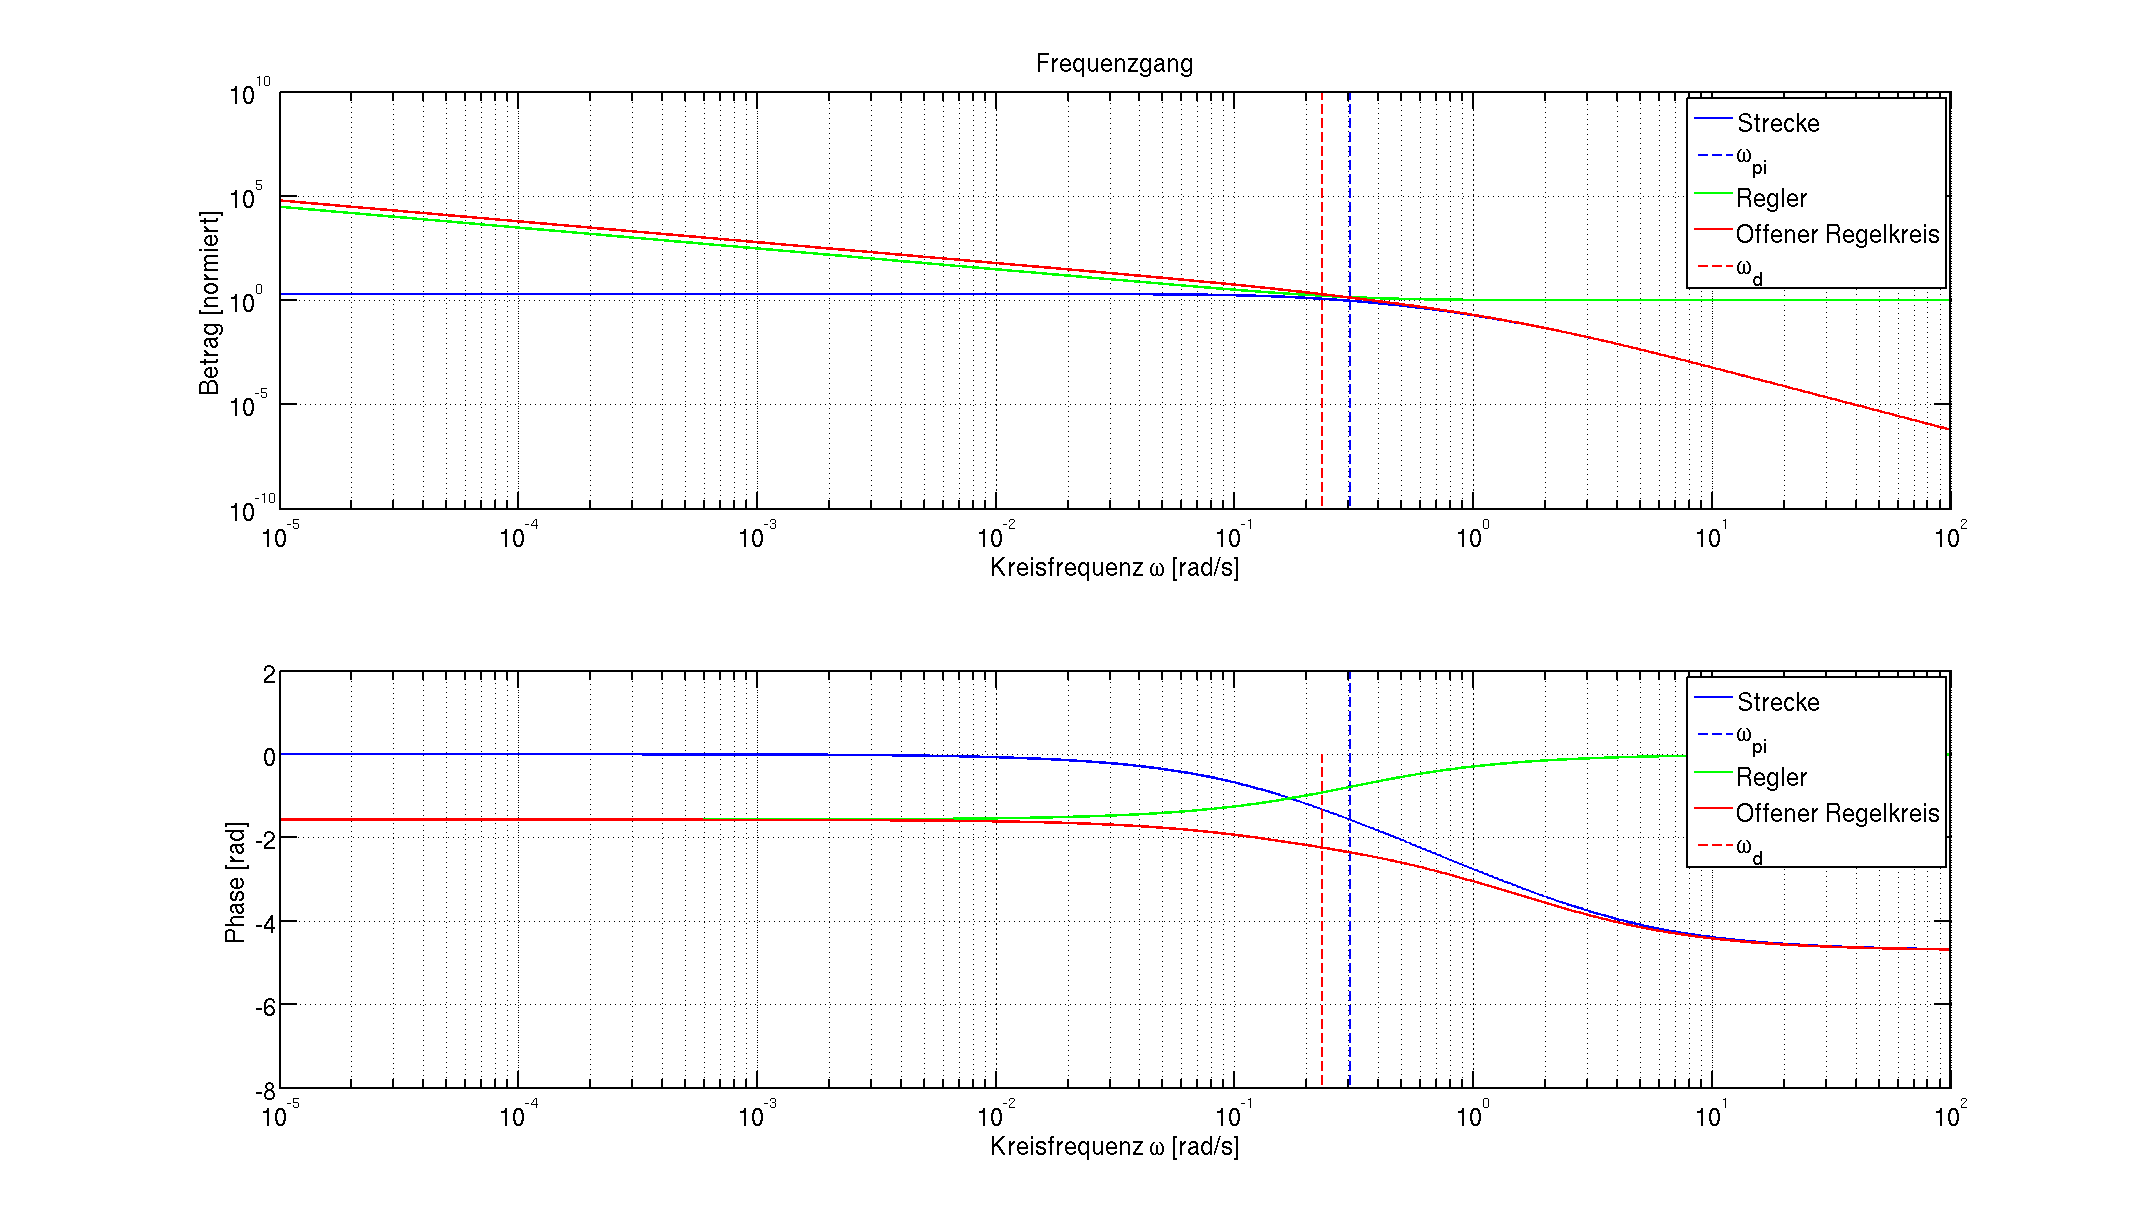
\includegraphics[width=\textwidth]{images/piBode.png}
    \caption{%
        Frequenzgang des Reglers (gr\"un), der  Strecke (blau) und des offenen
        Regelkreises (rot).
    }
    \label{fig:pi:all}
\end{figure}
\todo{Fix vertical line $\omega_d$}



\subsubsection*{PID-Regler}

Das schlussendliche Ziel ist die Bestimmung der Parameter $K_{rk}$, $T_{nk}$ und $T_{vk}$
in der Gleichung:

\begin{equation} \label{eq:pid:target}
    H_{rpid} = K_{rk} \cdot \biggl[ \frac{(1 + s \cdot T_{nk}) \cdot (1 + s \cdot T_{vk}) }{ s \cdot T_{nk} } \biggr]
\end{equation}

Analog  zum PID-Regler  wird zuerst  im  Phasengang der  Strecke die  Frequenz
$\omega_{pid}$  bestimmt, f\"ur  welche  die Phase  der Strecke  einen bestimmten
Wert aufweist, nur wird hier $-135\degree$ benutzt:

\begin{equation} \label{eq:pid:phi_s}
    \varphi_s(\omega_{pid}) = -135 \degree
\end{equation}

In unserem Beispiel ergibt dies:

\begin{equation} \label{eq:pid:omega_pid}
    \omega_{pid} = \SI{0.6714}{\per\second}
\end{equation}

Anschliessend wird  die Steigung des  Phasengangs $\varphi_s$ der  Strecke bei
der  Frequenz  $\omega_{pid}$  bestimmt. Ausgangspunkt  daf\"ur  ist  die  von
\code{p\_sani} bestimmte  \"Ubertragungsfunktion der Strecke  (siehe Gleichung
\ref{eq:transfer:plant}).

\begin{equation} \label{eq:transfer:plant:derivative}
    \frac{d\varphi_s}{d\omega} \biggr \rvert_{\omega=\omega_{pid}}
        = \frac{d(arg(H_s(j\omega)))}{d\omega} \biggr \rvert_{\omega=\omega_{pid}}
        = \SI{-1.5124}{\second}
\end{equation}
\todo{Einheit \"uberpr\"ufen}

Zwischen den Steigungen der Phasen des offenen Regelkreises ($\varphi_o$), der
Strecke ($\varphi_s$) und des Reglers ($\varphi_r$) gilt folgende Beziehung:

\begin{equation} \label{eq:pid:phi_sum}
    \varphi_o = \varphi_s + \varphi_r
\end{equation}

Da die Ableitung eine lineare Funktion ist, gilt somit auch: \todo{korrekte Begriffe}
\begin{equation} \label{eq:pid:dphi_sum}
    \frac{d\varphi_o}{d\omega} = \frac{d\varphi_s}{d\omega} + \frac{d\varphi_r}{d\omega}
\end{equation}

Diese Beziehungen  k\"onnen auch  gut in Abbildung  \ref{fig:pid_complete} von
Hand \"uberpr\"uft werden.

Es soll nun gelten:

\begin{equation} \label{eq:pid:dphi_o_target}
    \frac{d\varphi_o}{d\omega} \biggr \rvert_{\omega=\omega_{pid}} = - \frac{1}{2}
\end{equation}

Da   $\frac{d\varphi_s}{d\omega}$  durch   die  Strecke   gegeben  und   somit
unver\"anderlich ist, kann lediglich der Wert von $\frac{d\varphi_r}{d\omega}$
angepasst     werden,     damit     $\frac{d\varphi_o}{d\omega}$     Gleichung
\ref{eq:pid:dphi_o_target} erf\"ullt.

Dazu f\"uhrt man den Hilfsparameter $\beta$ ein, f\"ur den gilt:

\begin{gather} \label{eq:pid:beta:start}
    \begin{split}
        \frac{1}{T_{vk}} & = \frac{\omega_{pid}}{\beta} \\
        \frac{1}{T_{nk}} & = \omega_{pid} \cdot \beta  \\
                       0 & <  \beta \leq 1
    \end{split}
\end{gather}

Die  beiden Frequenzen  $\frac{1}{T_{vk}}$  und  $\frac{1}{T_{nk}}$ sind  also
symmetrisch  um den  Faktor $\beta$  gr\"osser bzw.  kleiner als  die Frequenz
$\omega_{pid}$. \todo{siehe Plot} Will man  $\beta$ von Hand bestimmen, trifft
man zuerst eine ``vern\"unftige'' Annahme, zum Beispiel:

\begin{equation} \label{eq:pid:beta:initial_value}
    \beta = 0.5
\end{equation}

Mit  diesem Startwert  bestimmt  man nun  $T_{nk}$  und ${T_{vk}}$. Die  somit
erhaltenen Werte setzt man in  Gleichung \ref{eq:pid:target} ein, zusammen mit
dem Wert f\"ur $\omega_{pid}$ aus Gleichung \ref{eq:pid:omega_pid}:

\begin{gather} \label{eq:pid:t_nk_t_vk_initial_results}
    \begin{split}
        {T_{vk}} & = \frac{\beta}{\omega_{pid}}  = \frac{0.5}{\SI{0.6714}{\per\second}}                   = \SI{0.7447}{\second} \\
        {T_{nk}} & = \frac{1}{\omega_{pid} \cdot \beta} = \frac{1}{\SI{0.6714}{\per\second} \cdot 0.5 }  = \SI{2.9789}{\second} \\
    \end{split}
\end{gather}

Eingesetzt in die Reglergleichung, vorerst mit $K_{rk} = 1$:

\begin{gather} \label{eq:pid:t_nk_t_vk_initial_results}
    \begin{split}
        H_{rpid} & = K_{rk} \cdot \biggl[ \frac{(1 + j\omega \cdot T_{nk}) \cdot (1 + j\omega \cdot T_{vk}) }{ j\omega \cdot T_{nk} } \biggr] \\
                 & = 1      \cdot \biggl[ \frac{(1 + j\omega \cdot \SI{2.9789}{\second}) \cdot (1 + j\omega \cdot \SI{0.7447}{\second}) }{ j\omega \cdot  \SI{2.9789}{\second}} \biggr]
    \end{split}
\end{gather}

Von dieser Gleichung bestimmt man nun den Phasengang und wertet danach dessen
Ableitung an der Stelle $\omega = \omega_{pid}$ aus:

\begin{gather} \label{eq:pid:phi_r_first_iteration}
    \begin{split}
        \varphi_s (j\omega)                                            & = arg(H_{rpid}(j\omega))        \\
        \frac{d\varphi_s}{d\omega} \biggr \rvert_{\omega=\omega_{pid}} & = \SI{1.1920}{\second}
    \end{split}
\end{gather}
\todo{Die zugeh\"orige Rechnung ist lange und m\"uhsam, allenfalls in Anhang? Ebenfalls: Einheit kontrollieren}


Setzt man dies in Gleichung \ref{eq:pid:phi_sum} ein, erh\"alt man:
\begin{gather} \label{eq:pid:phi_sum_result_iteration_one}
    \begin{split}
    \frac{d\varphi_o}{d\omega}       \biggr \rvert_{\omega=\omega_{pid}, \beta=0.5}
        & = \frac{d\varphi_s}{d\omega} \biggr \rvert_{\omega=\omega_{pid}}
        + \frac{d\varphi_r}{d\omega} \biggr \rvert_{\omega=\omega_{pid}, \beta=0.5} \\
        & = \SI{-1.5124}{\second} + \SI{1.1920}{\second} \\
        & = \SI{-0.3204}{\second} \\
        & > -\frac{1}{2}
    \end{split}
\end{gather}

Mit  $\beta  = 0.5$  erh\"alt  man  also eine  zu  hohe  Steigung des  offenen
Regelkreises   an    der   Stelle  $\omega_{pid}$,   folglich   muss   $\beta$
{\em{verkleinert}} werden.   Diese Berechnungen  werden nun mit  jeweils neuen
Werten  f\"ur  $\beta$  solange  wiederholt,  bis  die  Steigung  des  offenen
Regelkreises die gew\"unschte N\"ahe zu $-\frac{1}{2}$ aufweist.

Da die manuelle Iterierung dieses Prozesses enorm viel Zeit in Anspruch nimmt,
bietet  sich  hier  eine  Automatisierung  an. Die  Berechnung  mittels  eines
geeigneten Algorithmus in Matlab liefert schlussendlich folgendes Ergebnis:
\todo{Allenfalls Matlab-Algo in Anhang und Verweis}

\begin{gather} \label{eq:pid:beta_result}
    \begin{split}
        \beta    & = 0.2776 \\
        {T_{vk}} & = \frac{\beta}{\omega_{pid}}           = \SI{0.4134}{\second} \\
        {T_{nk}} & = \frac{1}{\omega_{pid} \cdot \beta}   = \SI{5.3656}{\second} \\
    \end{split}
\end{gather}

Sollte  man  f\"ur  $\beta$  einen komplexen  Wert  erhalten,  wird  $\beta=1$
gesetzt.\todo{Wie kann dies egtl. passieren?}

Diese  Werte setzt man nun in Gleichung \ref{eq:pid:target} ein. $K_{rk}$ wird
wie bei der Bestimmung von $\beta$ vorerst noch auf 1 gesetzt.

\begin{gather} \label{eq:pid:h_rpid_beta_result}
    \begin{split}
        H_{rpid} & = K_{rk} \cdot \biggl[ \frac{(1 + s \cdot T_{nk}               ) \cdot (1 + s \cdot T_{vk}               ) }{ s \cdot T_{nk}               } \biggr]
                   = 1      \cdot \biggl[ \frac{(1 + s \cdot \SI{5.3656}{\second} ) \cdot (1 + s \cdot \SI{0.4134}{\second} ) }{ s \cdot \SI{5.3656}{\second} } \biggr]
    \end{split}
\end{gather}

Zur Bestimmung von $K_{rk}$ wird nun der Frequenzgang des offenen Regelkreises
betrachtet. Dazu  multipliziert  man  wie  gehabt  die  \"Ubertragungsfunktion
der  Strecke   (siehe  Gleichung   \ref{eq:transfer:plant})  mit   der  soeben
bestimmten  provisorischen   \"Ubertragungsfunktion  des   Reglers  (Gleichung
\ref{eq:pid:h_rpid_beta_result}).

\begin{equation} \label{eq:pid:h_o_k_rk_one}
    H_{o}(j\omega) = H_{rpid}(j\omega) \cdot H_s(j\omega)
\end{equation}

Nun wird  die Durchtrittsfrequenz $\omega_d$  bestimmt, an welcher  der offene
Regelkreis eine  Verst\"arkung von $\SI{0}{\decibel} =  1$ aufweisen soll. Wie
auch  beim  PI-Regler  werden  wir   hier  ein  \"Uberschwingen  von  $16.3\%$
anstreben, womit gilt:

\begin{equation} \label{eq:pid:omega_d_target}
    \varphi_s(\omega_d) = \varphi_s = -128.5\degree
\end{equation}

Dieser Wert wird analog zum PI-Regler aus dem Phasengang des offenen Regelkreises
abgelesen. \todo{siehe Plot} Eine Nachrechnung mittels Matlab ergibt:


\begin{equation} \label{eq:pid:omega_d_target}
    \omega_d = \SI{0.5341}{\per\second}
\end{equation}

In einem letzten Schritt wird  nun der Amplitudengang des offenen Regelkreises
an der  Stelle $\omega_d$ gleich 1  gesetzt und diese Gleichung  nach $K_{rk}$
aufgel\"ost:

\begin{equation} \label{eq:pid:h_o_k_rk_one}
    \begin{split}
        A_{o}(j\omega_d)    & = | H_{o}(j\omega_d) |                            \\
                            & = | H_{rpid}(j\omega_d) \cdot H_s(j\omega_d) |    \\
                            & = \Biggl \rvert
                                    K_{rk}
                                    \cdot
                                    \biggl[ \frac{(1 + j\omega_d \cdot T_{nk}) \cdot (1 + j\omega_d \cdot T_{vk}) }{ j\omega_d \cdot T_{nk} } \biggr] \Biggr \rvert \\
                            & \cdot
                                \Biggl \rvert
                                    K_s
                                    \cdot \frac{1}{1 + j\omega_d \cdot T_1}
                                    \cdot \frac{1}{1 + j\omega_d \cdot T_2}
                                    \cdot \frac{1}{1 + j\omega_d \cdot T_2}
                                    \Biggr \rvert \\
                            & = 1
    \end{split}
\end{equation}

Mit den gegebenen und berechneten Werten:
\begin{gather} \label{eq:pid:h_o_k_rk_one}
    \begin{split}
        K_s         & = 2                        \\
        T_1         & = \SI{0.4134}{\second}     \\
        T_2         & = \SI{1.4894}{\second}     \\
        T_3         & = \SI{5.3655}{\second}     \\
        T_{nk}      & = \SI{5.3656}{\second}     \\
        T_{vk}      & = \SI{0.4134}{\second}     \\
        \omega_d    & = \SI{0.5341}{\per\second}
    \end{split}
\end{gather}

Dies liefert:

\begin{equation} \label{eq:pid:k_rk_result}
    K_{rk} = 1.83084
\end{equation}

Somit ist der Regler vollst\"andig bestimmt und hat folgende \"Ubertragungsfunktion:

\begin{equation} \label{eq:pid:result}
    H_{rpid}(s) = 1.83084 \cdot \biggl[ \frac{(1 + s \cdot \SI{5.3656}{\second} ) \cdot (1 + s \cdot \SI{0.4134}{\second} ) }{ s \cdot \SI{5.3656}{\second} } \biggr]
\end{equation}

Die Frequenzg\"ange der Strecke, des Reglers und des offenen Regelkreises:

\begin{figure}[h! width=\pagewidth]
    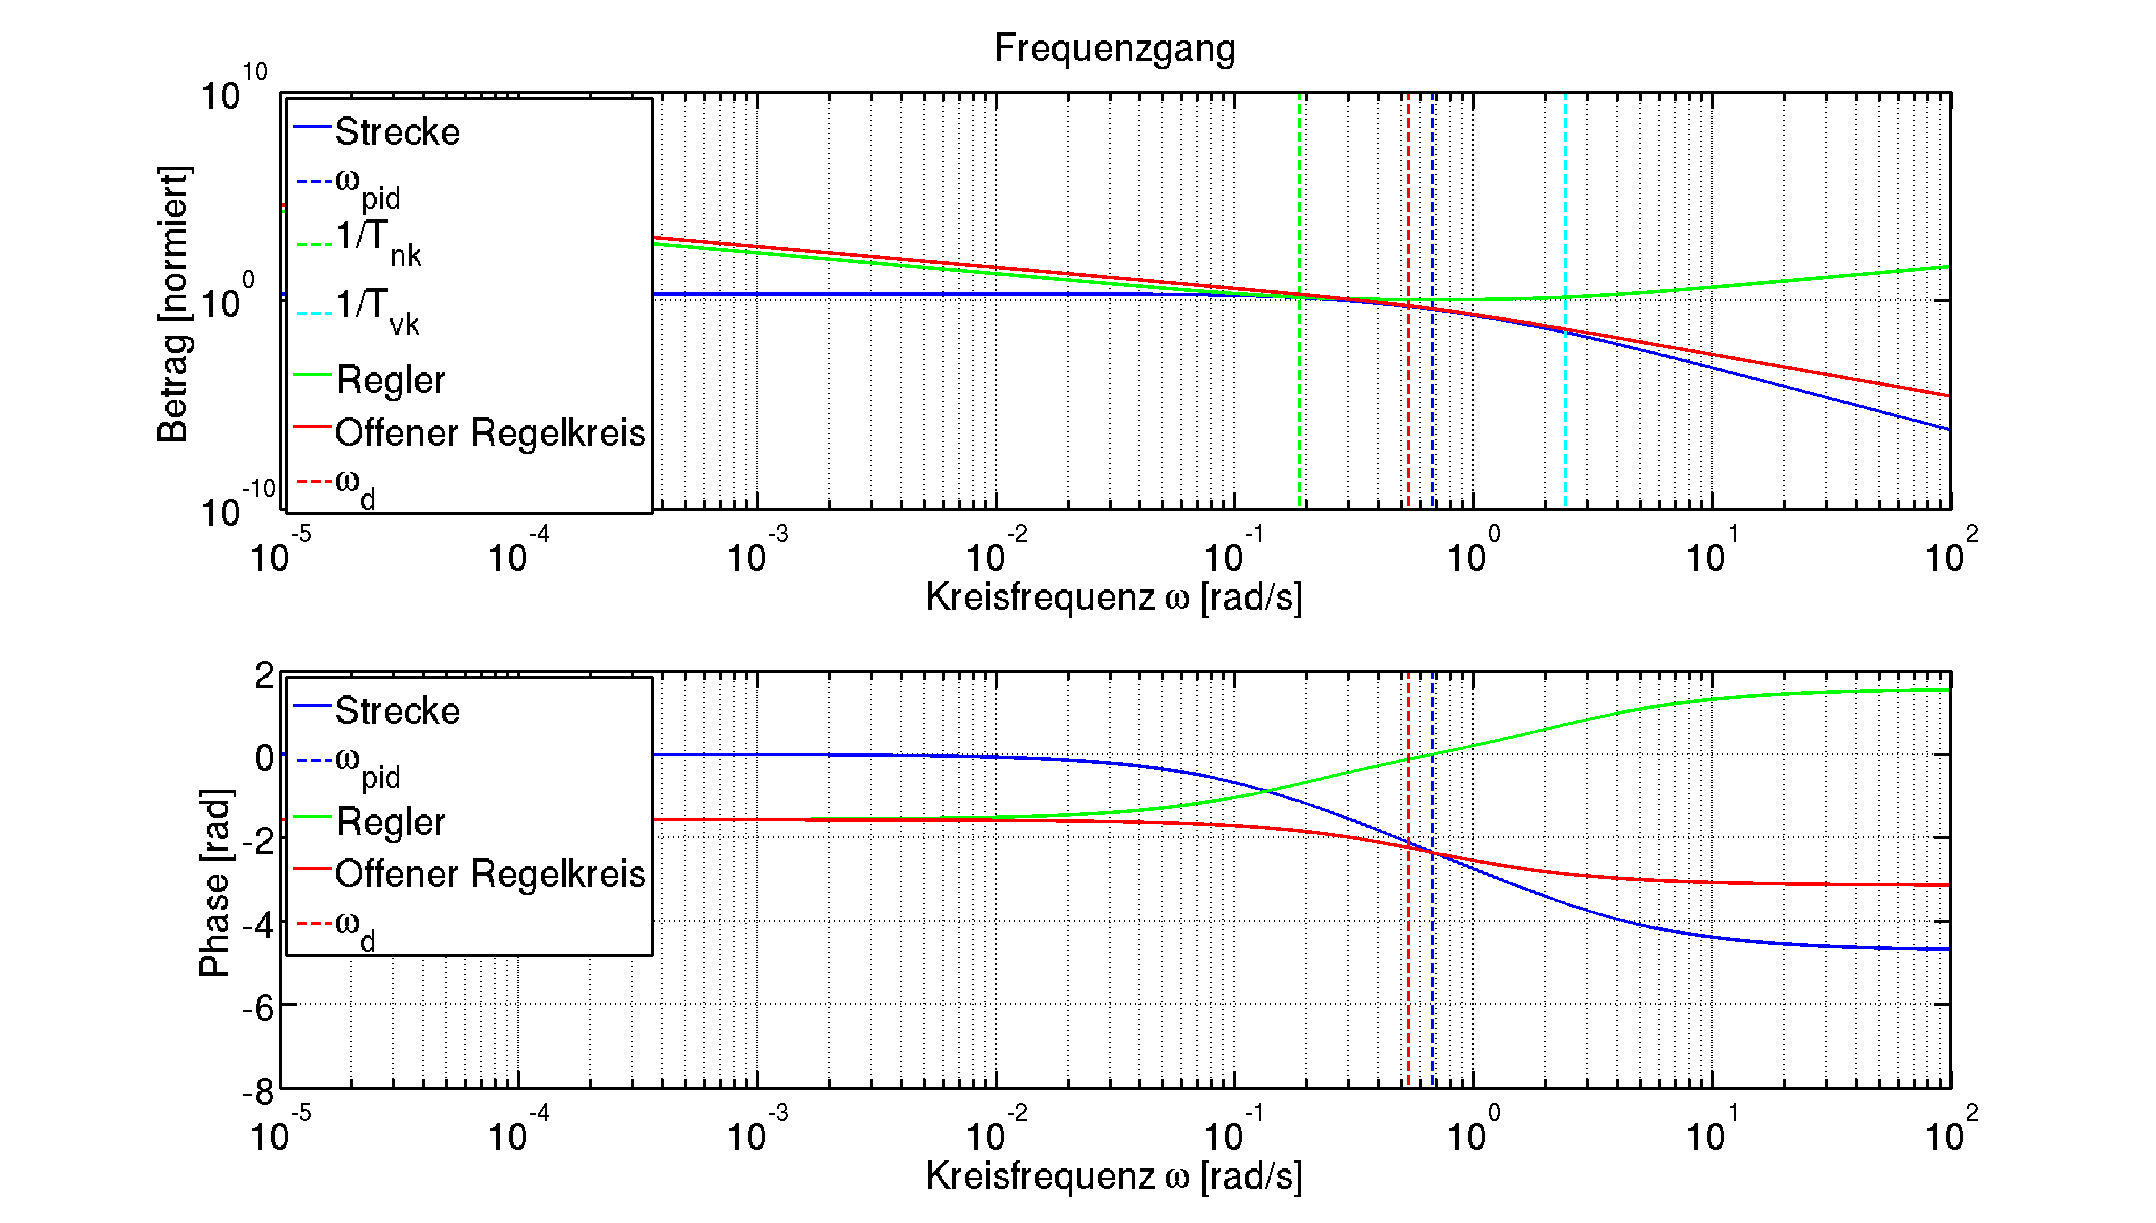
\includegraphics[width=\textwidth]{images/pidCompletePlot.png}
    \caption{%
        Frequenzgang der Strecke (blau), des  Reglers (gr\"un) und des offenen
        Regelkreises  (rot).  Ebenfalls  eingetragen  sind die  Reglerfrequenz
        $\omega_{pid}$,   die   beiden   Frequenzen   $\frac{1}{T_{vk}}$   und
        $\frac{1}{T_{nk}}$ sowie die Durchtrittsfrequenz $\omega_d$.
    }
    \label{fig:pid_complete}
\end{figure}
\clearpage
